\documentclass{article}

\usepackage[utf8]{inputenc}
\usepackage{graphicx}
\usepackage[margin=1in]{geometry}
\usepackage{subcaption}

\title{\vspace{30mm}EE382M: VLSI I \\ Monolithic 3D IC Basic Cell Library}

\author {
	Emily~Bragg,~Tengchieh~Huang\\
       	\em emily.bragg@utexas.edu,~tengchieh@utexas.edu\
}

\date{\today}

\begin{document}
\maketitle

\newpage
\section{Introduction}
3D integrated circuits (3DICs) are one potential advancement that will allow circuit designers to save area by having different parts of a design on different layers of silicon which are then bonded together. There are several different styles of 3DIC technology, but we will be focusing on monolithic 3DICs. We designed a standard cell library for 3DIC technology, and simulated the cells to determine the performances differences as compared to the standard version of each cell. 
\section{Technology Background}
\subsection{3D ICs} There are two common types of 3D ICs. The more common variety, which the library we plan to use was designed for, uses Through-Silicon Vias (TSVs) to connect layers, with each layer typically having full transistors. This allows vertical logic, but requires careful planning so as to ensure that the layers line up. Another issue with this approach is that a single TSV is very large relative to the cells it connects; at a 45nm technology node, the minimum width of a TSV is 6000nm ~\cite{NCSU}. This obviously cannot be used for fine-grained modifications to a design, and must be planned for when the design is initially made. 
\subsection{Monolithic 3D ICs} One way of avoiding the problem with TSV is through monolithic 3D IC technology. This technology is also a vertical technology, but it builds up very thin layers of devices instead of bonding them together. Instead of having TSVs, monolithic integration has 'monolithic inter-tier vias' (MIV). These MIVs, at 70nm, are a similar size to the contacts used at a 45nm technology node~\cite{ULTRA}, and thus can be used to design individual cells across multiple layers. They additionally have negligible parasitic capacitance. Because a significant portion of cell area comes from the necessary separation between the pwell and the nwell, by splitting the pull-up network and pull-down networks and putting each on a separate layer, we can achieve significantly smaller area without having to alter logic. We also considered doing the method presented in ~\cite{CELONCEL}; however, due to the limitations of the tools, the advantages of these method (stacking cells on top of other cells by layers to reduce wire lengths and delays across designs) would be difficult to illustrate.

\section{Specifications}
\subsection{Overview} We are designing a library of standard cells (listed in Table \ref{tab:cell_table}) for reducing area using monolithic 3D IC technology. Once completed, these cells should be able to be placed in a design andreduce the area by up to 40\% in the ideal case. This also should allow for less area consumed by routing, as routing can be run in the layer that has less area dedicated to logic (typically the same layer as the NMOS, due to the smaller transistor widths).

\begin{table}[ht]
\centering
\begin{tabular}{|c|c|} 
\hline
Cell & Sizes \\ \hline
AND & 2,3,4 \\ \hline
OR & 2,3, 4\\ \hline
NAND & 2, 3,4 \\ \hline
NOR & 2, 3, 4\\ \hline
AOI & 21, 22 \\ \hline
OAI & 21, 22 \\ \hline
INV & N/A \\ \hline
BUF & N/A \\ \hline
\end{tabular}
\caption{Cell Types and Sizes}
\label{tab:cell_table}
\end{table}

\subsection{Interface} The goal of cell design is to ensure that the inputs and outputs match identically with standard cell libraries of traditional technology. As such, each cell has the standard outputs. The primary difference is that the target library has VDD and GND rails stacked on separate layers, and as such they are not at opposing ends of the cell as they traditionally are in standard cells. All inputs and outputs come from the opposite side of the cell from the power and ground rails in our designs. 

\subsection{Design Targets} Our primary goal is area reduction, and we expect that using 3D IC technology can achieve area improvements approaching 50\% in the ideal case. However, we expect most of our better gains to be around 40\% less area, due to the overhead created by the MIVs. The best cases for area reduction come from gates that have equally sized PMOS and NMOS transistors; however, this is rarely the case (with size typically larger on the PMOS network), and even if it were, we could not achieve 50\% area reduction due to the MIV area. We plan to create reference versions of all of the standard cells, and the power and timing requirements for the reference versions are our design targets for the power and timing requirements of the 3D versions. 

\section{Design}
\subsection{Basic Architecture} The most basic goal of our design is to achieve the functionality of each standard cell. Because we used the technique outlined in ~\cite{ULTRA}, the PMOS and NMOS networks remained the same as they were in the standard cell, except for removing the poly between and replacing it with a contact to metal1. 
\subsection{Toolset} NCSU has a library for 3D ICs that we initially considered using. However, while it does support multiple layers, it has no functionality for MIVs (focusing rather on TSV-based ICs). This meant two things for our design. Firstly, if we built our designs using the 3D IC library provided, there would be no way of achieving power and timing simulation, as TSV technology has radically different effects. Secondly, TSVs would dominate the area of any cell, and thus we would not be able to get valid area results either. The only advantage this path would have had would be for purposes of simulating the logic, which was basic and thus would not be important information. \\ 
We instead decided to utilize the standard 45nm NCSU libraries. While this does not support laying directly, we were able to simulate the effect of the MIV by separating the layers with a metal1 wire, with the length calculate to provide the same resistance as the MIV would, for power and timing simulations. Additionally, as the contacts connecting the poly to the wire are within 5nm of the size of a MIV, we can accurately measure the area. This approach allowed us to calculate the area, power, and timing achievable if we had tools that supported the technology. 
	\begin{figure}[t]
		\centering
		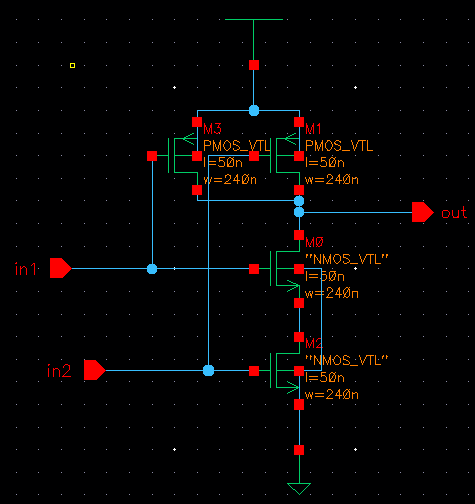
\includegraphics[width=7cm]{step1}
  		\caption{NAND2 Schematic}
		\label{step1}
	\end{figure}		
\begin{figure}[h]
\centering
\parbox{8cm}{
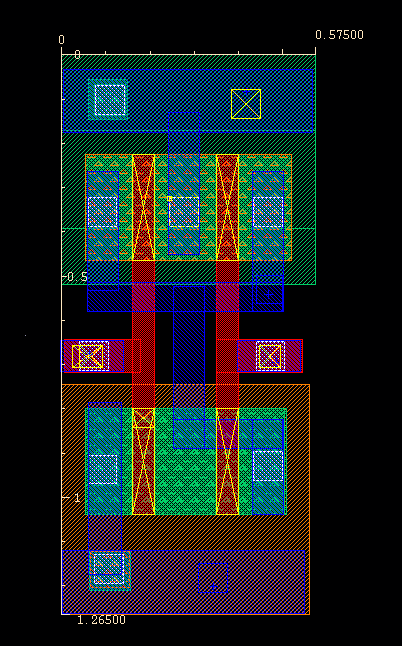
\includegraphics[width=4cm]{step3}
  \caption{NAND2 Layout}
\label{step3}}
\qquad
\begin{minipage}{7cm}
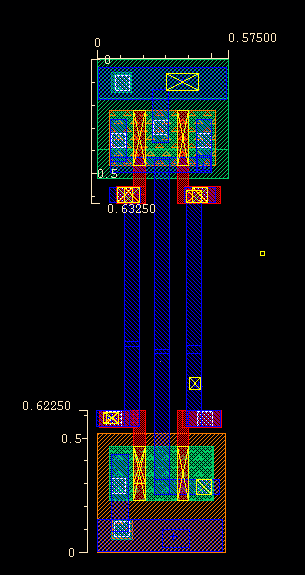
\includegraphics[width=4cm]{3d_layout}
  \caption{Simulated 3D NAND2 Layout - Middle wires shortened for figure visibility}
\label{3d_layout}
\end{minipage}
\end{figure}

\subsection{Design Flow} To illustrate our procedure, here are the steps taken for a NAND2 gate. 
	\begin{enumerate}
		\item Create a schematic (Fig.~\ref{step1})
		\item Generate the pins from the schematic
		\item Create a layout for the standard cell (Fig.~\ref{step3})
		\item Take the standard cell layout and remove the interconnecting polysilicon
		\item Add a 65nm by 3420nm metal1 connection between the poly contacts and the inputs. This size was chosen by calculating the wire length necessary, when created from a material with the resistivity of metal1 (.25$\Omega$ / square) ~\cite{NCSU}, to simulate a MIV resistance of 20 $\Omega$ \cite{ULTRA} . We chose 65nm width to minimize the required length.  This is shown in Figure ~\ref{3d_layout}.
		\item Measure each half of the cell (the 3D IC area is equal to the max of the two sizes)
		\item Simulate the 3D version of the cell pre- and post- layout to determine the power and timing. Timing is shown for both rising and falling worst case scenarios for planar (Figures ~\ref{rising} and ~\ref{falling}) and 3D (Figures ~\ref{3d_rising} and ~\ref{3d_falling}) designs.
	\end{enumerate}
\begin{figure}
\centering
\parbox{8cm}{
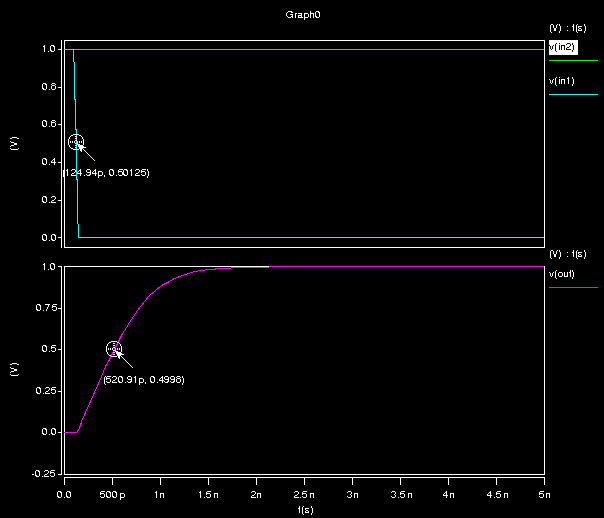
\includegraphics[width=7cm]{rising}
  \caption{Worst-case NAND2 Rising Time}
\label{rising}}
\qquad
\begin{minipage}{7cm}
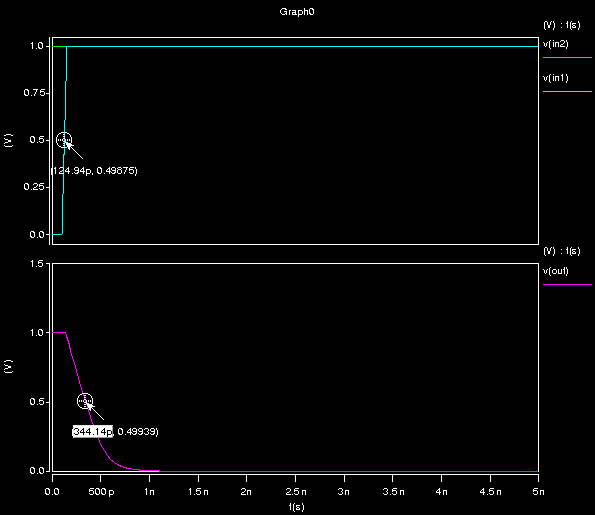
\includegraphics[width=7cm]{falling}
  \caption{Worst-case NAND2 Falling Time}
\label{falling}
\end{minipage}
\end{figure}

\begin{figure}
\centering
\parbox{8cm}{
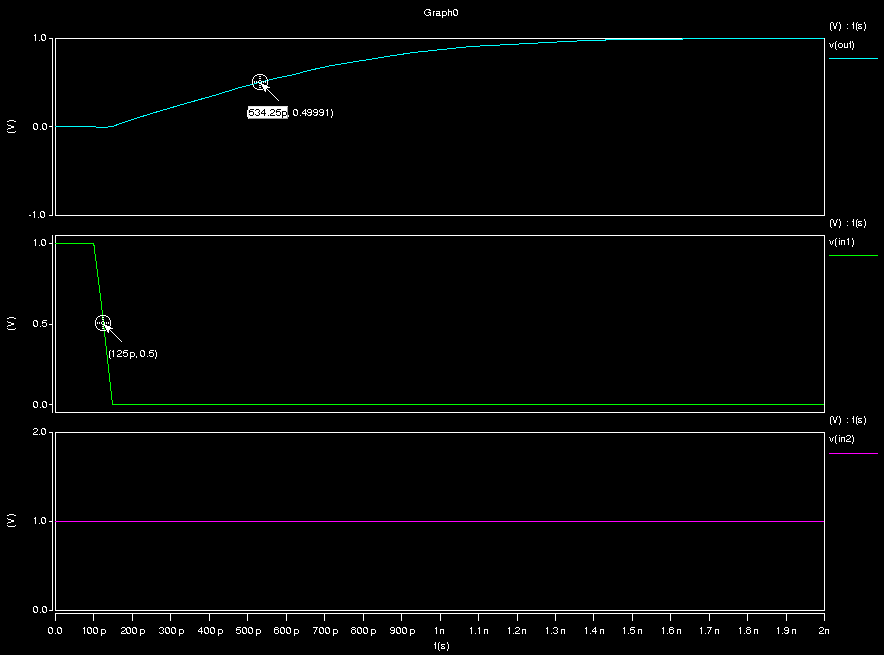
\includegraphics[width=7cm]{3d_rising}
  \caption{Worst-case NAND2\_3D Rising Time}
\label{3d_rising}}
\qquad
\begin{minipage}{7cm}
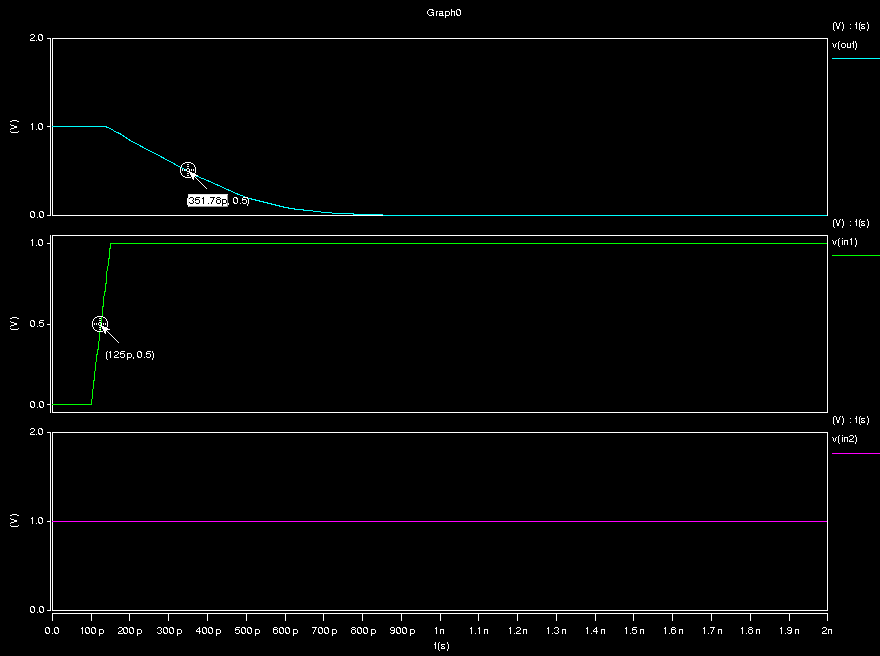
\includegraphics[width=7cm]{3d_falling}
  \caption{Worst-case NAND2\_3D Falling Time}
\label{3d_falling}
\end{minipage}
\end{figure}
\subsection{Optimization Techniques} We employed the standard optimization techniques used for standard cell libraries, as the pull-up and pull-down networks remain intact. These include sizing the transistors so that they are balanced, adding additional pins on the larger transistors to reduce the resistance from the contacts, and carefully routing the metal1 so as to avoid unnecessary area due to routing. The last one is particularly relevant, as space that would have been available between transistors due to minimum distances between wells is no longer available. One unique advantage that monolithic 3D IC technology gives us is the ability to reduce the length of the poly. As it notes in ~\cite{ULTRA}, the unit resistance of polysilicon is significantly higher than that of metal; by only having polysilicon on the transistor and not forming a wire between them, we can reduce the internal wire resistance. This counteracts the additional resistance provided by the MIV, producing what we anticipate to be a negligible timing difference.  
\subsection{Naming Conventions} Our naming conventions were to have either \textless CELLNAME\textgreater \textless CELLSIZE\textgreater, for a standard version of a cell, or \textless CELLNAME\textgreater \textless CELLSIZE\textgreater\_3D, for the version that has the additional wiring to simulate a 3D IC. 
\subsection{Issue Tracking} We kept track of the cells through git, using it to track progress, bugs, to-do items, and notes on each design as we worked on them. 


\section{User Document}
\subsection{Using 3DMI Standard Cells}
The 3DMI standard library has similar design concept with conventional planar process standard library. The biggest difference is it separate NMOS and PMOS transistors into two layers, which can be used to reduce chip area, global wire routing length and even provide new way of circuit design.
  In this library, we put all the PMOS transistors and power rail (VDD) into the bottom layer, because normally PMOS transistors occupy larger area. For the bottom layer, we apply 4BM metal layer stack [Ultra High Density Logic Designs …] which adds 3 metal layers to the bottom tier. In other word, there are total 4 local metal layers available on the bottom tier. It is a good choice because as we mentioned, in this library PMOS transistors are located in the bottom tier. With more local metal line, it could bring more convenience when routing in tight space.
  For each cell, there is  always one side for the connection of  inter-tier vias (MIVs). Therefore, routing should be more careful when wires are close to the edge. Another important thing is when choosing cells, some cells could be more  favorable than others, especially for cells have similar NMOS and PMOS area, which will be discussed later.

\subsection{Standard Cell List}
  We choose total 20 standard cells, including an inverter chain to test the potential problems caused by monolithic 3D integration. All of the cells should be sufficient for normal design, and could be useful for testing most of the circuits using 3DMI process. In order to compare the differences between 2D and 3D process, we construct both type with the same floorplanning mechanism which can help easily understand the advantages and disadvantages among two strategies.


\begin{table}
\centering
\begin{tabular}{|c|c|c|} 
\hline
Category&Number of cells&Cell Names \\ \hline
buffer&3&INV, BUF, INV\_CHAIN \\ \hline
logic&16&NAND2/3/4, NOR2/3/4,  \\ \hline
      &&  AND2/3/4, OR2/3/4, \\ \hline  
    &&AOI21, OAI21, AOI22, OAI22 \\ \hline
\end{tabular}
\label{tab:2d_cell_list}
\caption{2D Cells Created}
\end{table}

\begin{table}
\centering
\begin{tabular}{|c|c|c|} 
\hline
Category&Number of cells&Cell Names \\ \hline
buffer&3&INV\_3D, BUF\_3D, INV\_CHAIN\_3D \\ \hline
logic&16&NAND2/3/4\_3D, NOR2/3/4\_3D, \\ \hline
        &&AND2/3/4\_3D, OR2/3/4\_3D,  \\ \hline
    &&AOI21\_3D, OAI21\_3D, AOI22\_3D, OAI22\_3D \\ \hline
\end{tabular}
\label{tab:3d_cell_list}
\caption{3D Cells Created}
\end{table}


\subsection{Cell Area}
  One of the most obvious benefit of using 3D ICs is that they can reduce area of the chips or SoCs by stacking the circuits and growing vertically. Here we not only provide the cell area of monolithic 3D standard cells but also  the cell area for 2D standard cells. Therefore, you can use the tables to calculate how much area could be saved by using 3DMI.

\begin{table}
\centering
\begin{tabular}{|c|c|c|c|} 
\hline
cell names&area in 2D(um\^2)&area in 3DMI(um\^2)&difference percentage \\ \hline
INV&0.4151&0.2352&42.6\\ \hline
BUF&0.8483&0.4828&43.5\\ \hline
INV\_CHAIN&&& \\ \hline
NAND2&0.7242&0.4531&37.5\\ \hline
NAND3&1.0356&0.5946&43.5\\ \hline
NAND4&1.3523&0.7229&46.5\\ \hline
NOR2&0.7943&0.5304&29.4\\ \hline
NOR3&1.2288&0.8661&29.5\\ \hline
NOR4&1.7825&1.3195&26\\ \hline
AND2&1.1866&0.7102&41\\ \hline
AND3&1.5595&0.88&43.6\\ \hline
AND4&1.9815&1.179&40.5\\ \hline
OR2&1.3298&0.844&36.5\\ \hline
OR3&1.4506&1.2953&10.7\\ \hline
OR4&2.1974&1.792&18.4\\ \hline
AOI21&1.125&0.6244&44.2\\ \hline
AOI22&1.675&0.9165&45.3\\ \hline
OAI21&1.1306&0.6242&44.8\\ \hline
OAI22&1.9163&0.9237&51.6\\ \hline
\end{tabular}
\label{tab:nmos_area}
\caption{Total Area Comparison}
\end{table}

The following table provides the area of PMOS transistors and NMOS transistors in a single 3D standard cell. We can see which cells are more competitive when applied on 3D technology.
\begin{table}
\centering
\begin{tabular}{|c|c|c|c|} 
\hline
cell names&area of PMOS(um\^2)&area of NMOS(um\^2)&difference percentage\\ \hline
INV&0.2352&0.1925&22.2\\ \hline
BUF&0.4828&0.37&30.5\\ \hline
INV\_CHAIN&&&\\ \hline
NAND2&0.4531&0.3516&28.9\\ \hline
NAND3&0.5946&0.5547&71.9\\ \hline
NAND4&0.7229&0.7031&28.2\\ \hline
NOR2&0.5304&0.336&57.9\\ \hline
NOR3&0.8661&0.4615&87.7\\ \hline
NOR4&1.3195&0.6867&92.1\\ \hline
AND2&0.7102&0.6137&15.7\\ \hline
AND3&0.8158&0.88&7.3\\ \hline
AND4&0.9675&1.179&17.9\\ \hline
OR2&0.844&0.5688&48.4\\ \hline
OR3&1.2953&0.6891&88\\ \hline
OR4&1.792&0.8112&121\\ \hline
AOI21&0.6244&0.4894&27.6\\ \hline
AOI22&0.9165&0.5694&61\\ \hline
OAI21&0.6242&0.5527&12.9\\ \hline
OAI22&0.9237&0.7056&30.9\\ \hline

\end{tabular}
\caption{PMOS Area Comparison}
\label{tab:pmos_area}
\end{table}
\subsection{Cell Delay}
  The following table contains Presim, Postsim for both planar and monolithic 3D rising and falling time. Assume output capacitance is 50 fF. For 4BM metal layer stack we applied, the average resistance for a single stacked via is 20 ohms, and parasitic capacitance
 is 0.123 fF. After calculating and spice simulation, we found that metal 1 wire which is 3.42um long and 65 nm wide can fit the requirement well. As the extracted nettles files shows:

\begin{verbatim}
.subckt PM\_AND2\_OUT 3 7 8
c10 3 0 0.0371754f
r11 7 8 1.43133
r12 3 7 1.634
.ends

.subckt PM\_AND2\_3D\_OUT 4 8 12
c14 12 0 0.00285922f
c15 8 0 0.0134125f
c16 4 0 0.169493f  
r17 12 14 0.220645
r18 12 13 0.0980645
r19 8 14 0.975333
r20 4 13 19.304   
.ends
\end{verbatim}


  PM\_AND2\_OUT and PM\_AND2\_3D\_OUT are the same net in an AND2 cell, and the only difference is PM\_AND2\_3D\_OUT is connected to a 3.42 um metal 1 wire. You can find that C16 and r20 are quite close to our desired value. Since the parasitic resistance and capacitance of 3DMI stacking vias are not large, we think that it would be sufficient for the simulation.

\begin{table}
\centering
\begin{tabular}{|c|c|c|} 
\hline
cell names&rising time(ps)&falling time(ps) \\ \hline
INV&376.3&242.8 \\ \hline
BUF&383.65&263.52 \\ \hline
NAND2&383.94&212.3 \\ \hline
NAND3&386.24&201.86 \\ \hline
NAND4&390.49&197.51 \\ \hline
NOR2&409.65&235.72 \\ \hline
NOR3&431.36&263.98 \\ \hline
NOR4&446.26&268.06 \\ \hline
AND2&388.24&144.2 \\ \hline
AND3&392.82&110.57 \\ \hline
AND4&396.34&96.91 \\ \hline
AOI21&411.6&219.26 \\ \hline
AOI22&333&224.94 \\ \hline
OAI21&446.27&218.06 \\ \hline
OAI22&417.16&160.18 \\ \hline
\end{tabular}
\caption{Pre-layout Simulation}
\label{tab:prelayout}
\end{table}

\begin{table}
\centering
\begin{tabular}{|c|c|c|} 
\hline
cell names&rising time(ps)&falling time (ps) \\ \hline
INV&383.5&249.72 \\ \hline
BUF&394.09&270.84 \\ \hline
NAND2&396&219 \\ \hline
NAND3&413&213 \\ \hline
NAND4&435.65&212 \\ \hline
NOR2&419.79&262.17 \\ \hline
NOR3&454.44&279.22 \\ \hline
NOR4&488.38&301.18 \\ \hline
AND2&404.23&168.23 \\ \hline
AND3&414.82&163.74 \\ \hline
AND4&427.33&158.24 \\ \hline
AOI21&432.26&228.9 \\ \hline
AOI22&362.22&238.24 \\ \hline
OAI21&469.83&229.28 \\ \hline
OAI22&446.02&184.48 \\ \hline
\end{tabular}
\caption{Post-layout Simulation for 2D cells}
\label{tab:2postlayout}
\end{table}

\begin{table}
\centering
\begin{tabular}{|c|c|c|} 
\hline
cell names&rising time(ps)&falling time(ps) \\ \hline
INV&400.1&263.35 \\ \hline
BUF&410.3&283.51 \\ \hline
NAND2&409.25&227.25 \\ \hline
NAND3&428.65&221.3 \\ \hline
NAND4&451.14&223.65 \\ \hline
NOR2&436.55&273.12 \\ \hline
NOR3&471.58&290.01 \\ \hline
NOR4&506.42&312.27 \\ \hline
AND2&418.83&187.3 \\ \hline
AND3&429.62&180.12 \\ \hline
AND4&441.7&172.4 \\ \hline
AOI21&438.23&232 \\ \hline
AOI22&357.76&240.43 \\ \hline
OAI21&471.77&232.6 \\ \hline
OAI22&450.39&186.41 \\ \hline
\end{tabular}
\caption{Post-layout Simulation for 3D cells}
\label{tab:3postlayout}
\end{table}




\section{Testing}\label{sec:testing}
%testing methods, bugs encountered, traces applied

\section{Optimization}
\subsection{Optimizing Individual Cells}
Individual cells were primarily optimized using prior knowledge, as the design process (as noted in Section 3) does not differ significantly from the standard process. The methods that we used have all been thoroughly investigated in Lab 1 of this semester, and thus are not shown in detail. We used multiple contacts for all of the cells that had transistors large enough to fit multiple contacts, to reduce the resistance. Additionally, all transistors were sized to have 2:1 PMOS:NMOS transistors, to minimize delay. 

\subsection{Using Monolithic 3D ICs to Optimize Full Designs} The more interesting problem is how to use these completed cells to optimize existing designs. There are several facets, which we will analyze here; without support from the tools, it is difficult or impossible to show these in an actual design. 
\begin{enumerate}
	\item \textbf{Total Area} The biggest optimization goal of using 3D ICs is to reduce area. In the instances of balanced networks, as is shown in Section ~\ref{sec:testing}, the area saving can approach 40 -- 50 \% on individual cells. However, the more optimal the split between the two sections is, the less room is left for routing, and thus cells must be spaced out to allow for wires. If we assume an optimal gate (using the NAND2 numbers from above) that must route wires, the area savings goes down by 130nm for every second wire added (as they can be split between layers if there are an even number). For a NAND2 gate, that is equivalent to a third of the area savings for each additional wire. 
	\item \textbf{Routing} Another interesting case, and a more realistic one, is that the user has a balance of cell sizes and types. In this case, while the overall area savings are less, you can hide the routing overhead in the underutilized layer (typically with the NMOS, though the routing can also use MIVs to switch to the other layer if it becomes advantageous). This can help mitigate the pressure on routing. Designs have been found by ~\cite{ULTRA} to approach 40\% reduction in area, even with the additional difficulties of routing. 

\end{enumerate}

\newpage

\clearpage
\section{Cell Layouts} 

\begin{figure}[ht]
\centering
\parbox{8cm}{
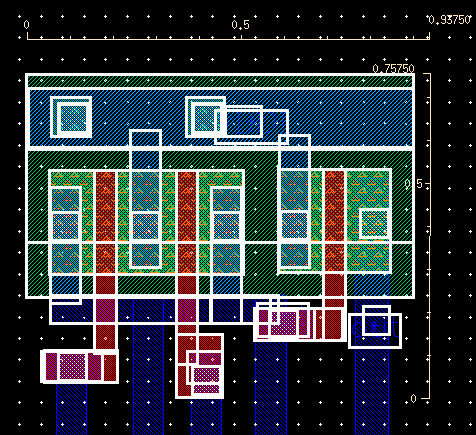
\includegraphics[width=7cm]{final_cells/AND2_PMOS}
  \caption{AND2 Pull-up Network}
\label{fig:AND2_pmos}}
\qquad
\begin{minipage}{7cm}
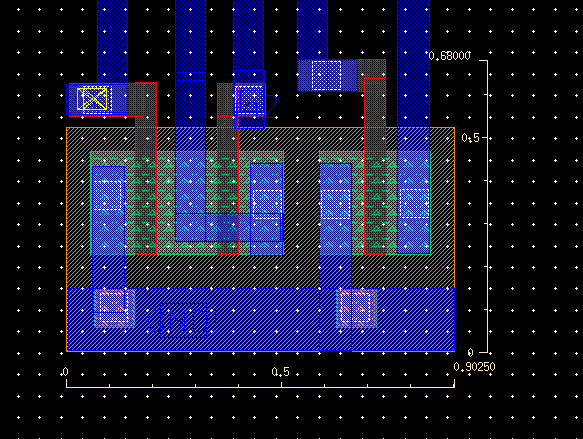
\includegraphics[width=7cm]{final_cells/AND2_NMOS}
  \caption{AND2 Pull-down Network}
\label{fig:AND2_nmos}
\end{minipage}
\end{figure}

\begin{figure}[ht]
\centering
\parbox{8cm}{
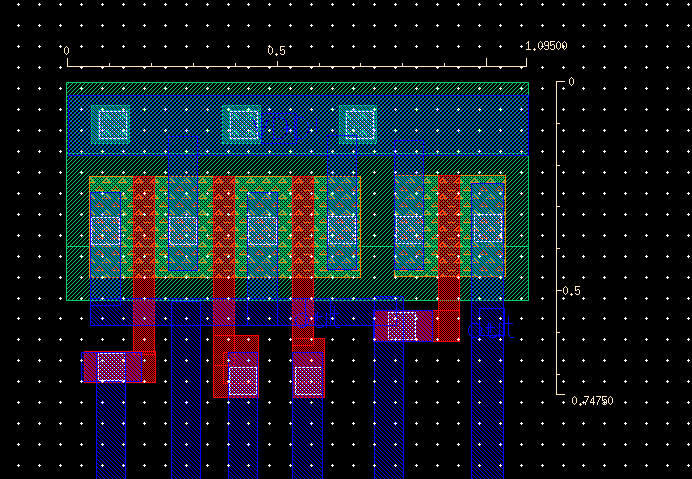
\includegraphics[width=7cm]{final_cells/AND3_PMOS}
  \caption{AND3 Pull-up Network}
\label{fig:AND3_pmos}}
\qquad
\begin{minipage}{7cm}
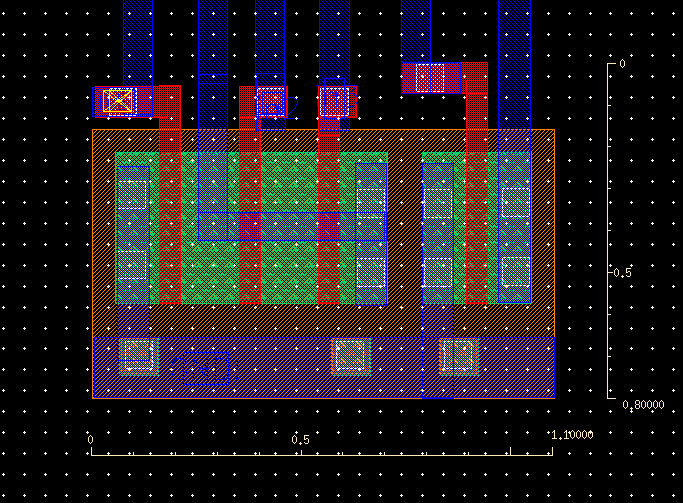
\includegraphics[width=7cm]{final_cells/AND3_NMOS}
  \caption{AND3 Pull-down Network}
\label{fig:AND3_nmos}
\end{minipage}
\end{figure}


\begin{figure}[ht]
\centering
\parbox{8cm}{
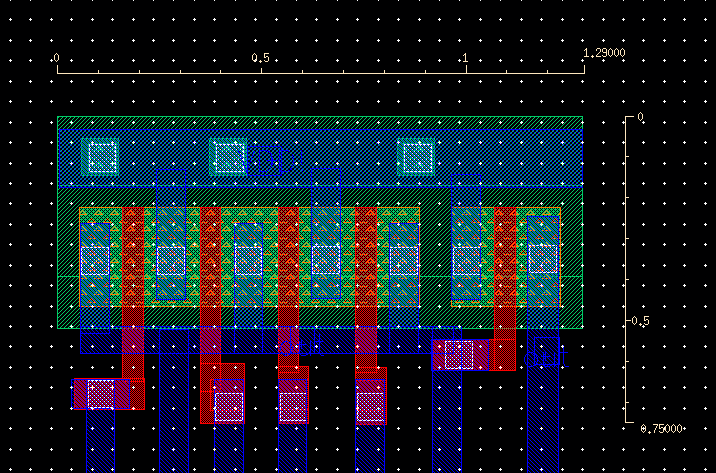
\includegraphics[width=7cm]{final_cells/AND4_PMOS}
  \caption{AND4 Pull-up Network}
\label{fig:AND4_pmos}}
\qquad
\begin{minipage}{7cm}
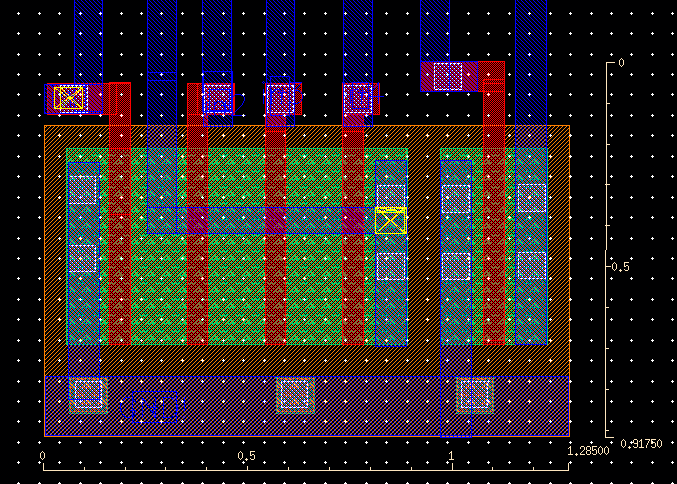
\includegraphics[width=7cm]{final_cells/AND4_NMOS}
  \caption{AND4 Pull-down Network}
\label{fig:AND4_nmos}
\end{minipage}
\end{figure}

\begin{figure}[ht]
\centering
\parbox{8cm}{
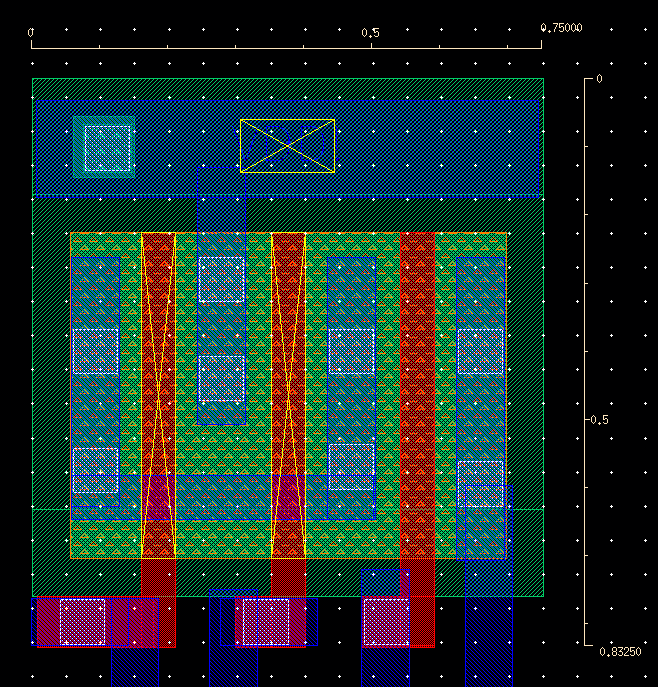
\includegraphics[width=7cm]{final_cells/AOI21_PMOS}
  \caption{AOI21 Pull-up Network}
\label{fig:AOI21_pmos}}
\qquad
\begin{minipage}{7cm}
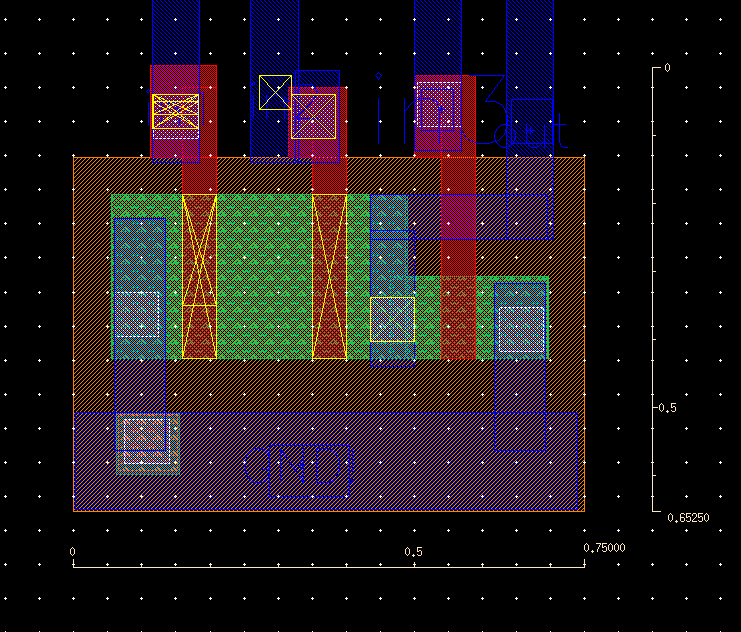
\includegraphics[width=7cm]{final_cells/AOI21_NMOS}
  \caption{AOI21 Pull-down Network}
\label{fig:AOI21_nmos}
\end{minipage}
\end{figure}

\begin{figure}[ht]
\centering
\parbox{8cm}{
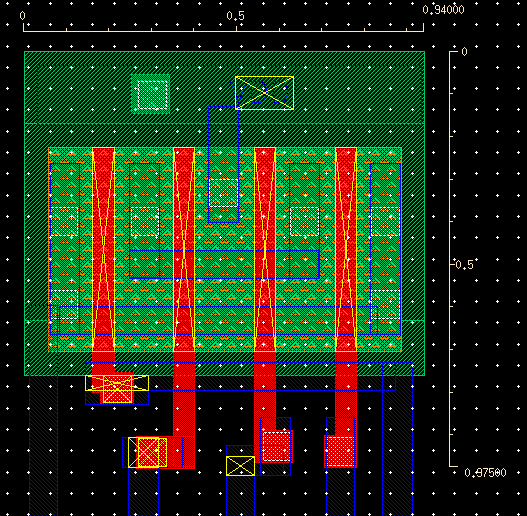
\includegraphics[width=7cm]{final_cells/AOI22_PMOS}
  \caption{AOI22 Pull-up Network}
\label{fig:AOI22_pmos}}
\qquad
\begin{minipage}{7cm}
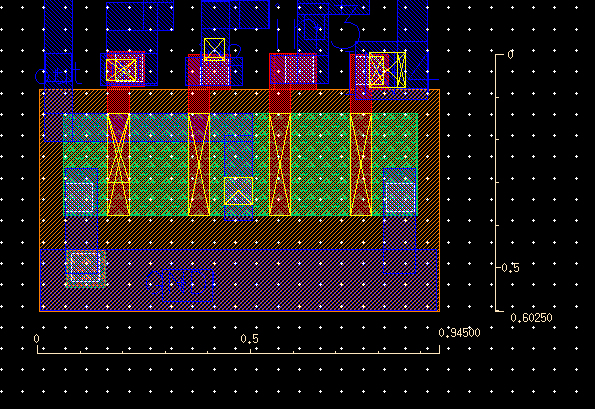
\includegraphics[width=7cm]{final_cells/AOI22_NMOS}
  \caption{AOI22 Pull-down Network}
\label{fig:AOI22_nmos}
\end{minipage}
\end{figure}

\begin{figure}[ht]
\centering
\parbox{8cm}{
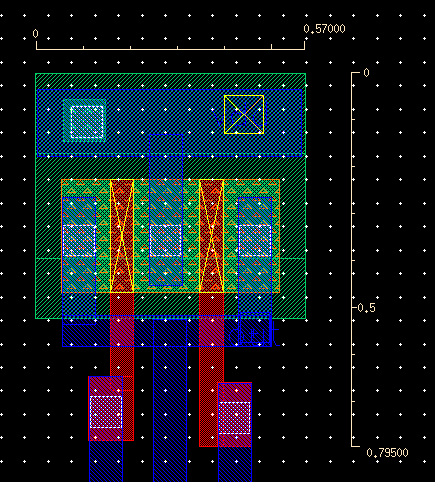
\includegraphics[width=7cm]{final_cells/NAND2_PMOS}
  \caption{NAND2 Pull-up Network}
\label{fig:NAND2_pmos}}
\qquad
\begin{minipage}{7cm}
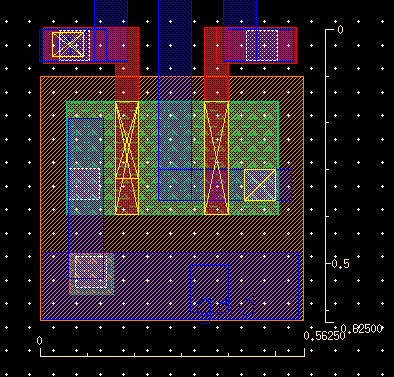
\includegraphics[width=7cm]{final_cells/NAND2_NMOS}
  \caption{NAND2 Pull-down Network}
\label{fig:NAND2_nmos}
\end{minipage}
\end{figure}

\begin{figure}[ht]
\centering
\parbox{8cm}{
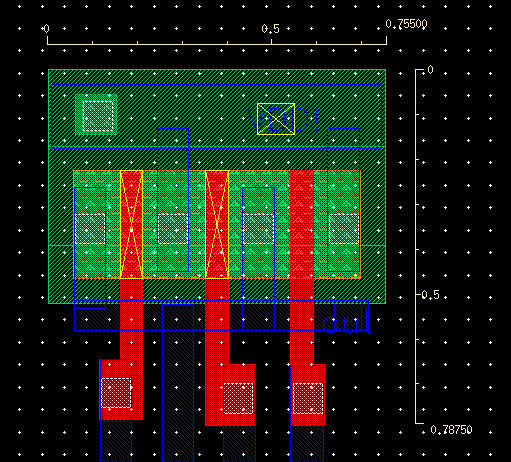
\includegraphics[width=7cm]{final_cells/NAND3_PMOS}
  \caption{NAND3 Pull-up Network}
\label{fig:NAND3_pmos}}
\qquad
\begin{minipage}{7cm}
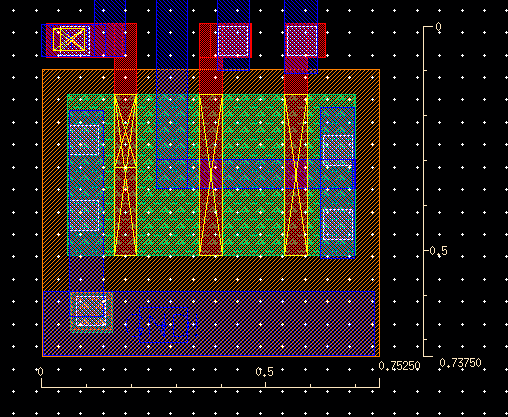
\includegraphics[width=7cm]{final_cells/NAND3_NMOS}
  \caption{NAND3 Pull-down Network}
\label{fig:NAND3_nmos}
\end{minipage}
\end{figure}

\begin{figure}[ht]
\centering
\parbox{8cm}{
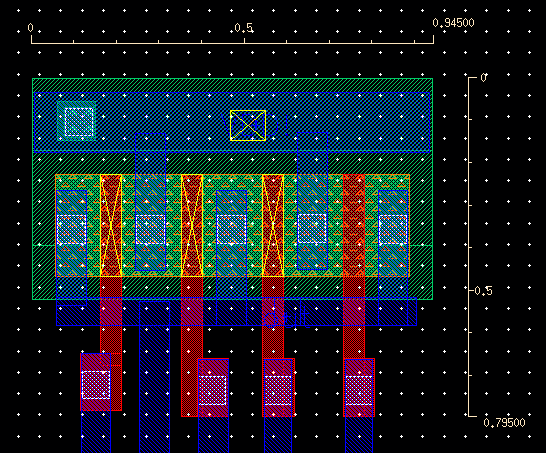
\includegraphics[width=7cm]{final_cells/NAND4_PMOS}
  \caption{NAND4 Pull-up Network}
\label{fig:NAND4_pmos}}
\qquad
\begin{minipage}{7cm}
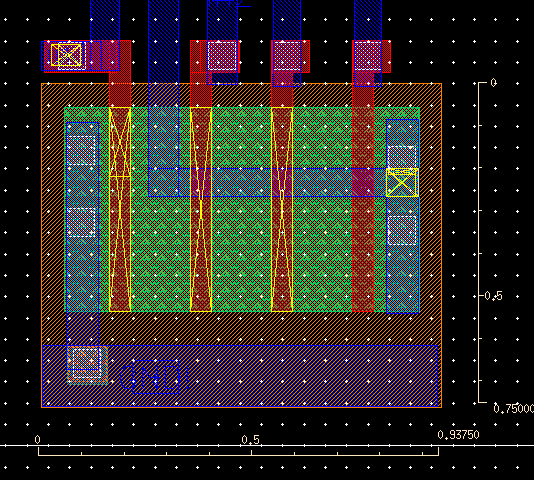
\includegraphics[width=7cm]{final_cells/NAND4_NMOS}
  \caption{NAND4 Pull-down Network}
\label{fig:NAND4_nmos}
\end{minipage}
\end{figure}

\begin{figure}[ht]
\centering
\parbox{8cm}{
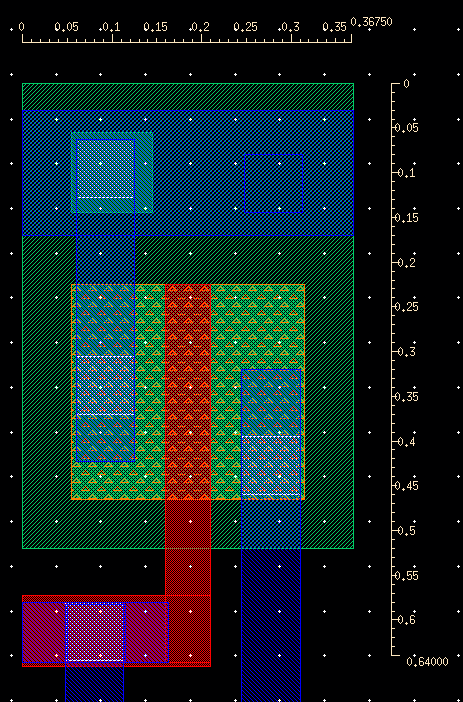
\includegraphics[width=7cm]{final_cells/INV_PMOS}
  \caption{INV Pull-up Network}
\label{fig:INV_pmos}}
\qquad
\begin{minipage}{7cm}
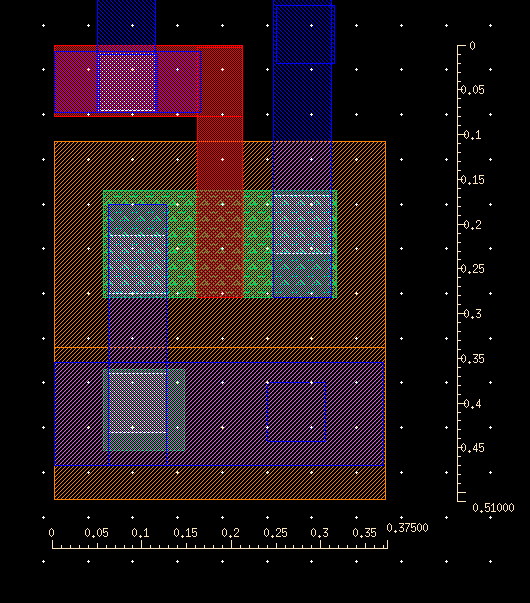
\includegraphics[width=7cm]{final_cells/INV_NMOS}
  \caption{INV Pull-down Network}
\label{fig:INV_nmos}
\end{minipage}
\end{figure}

\begin{figure}[ht]
\centering
\parbox{8cm}{
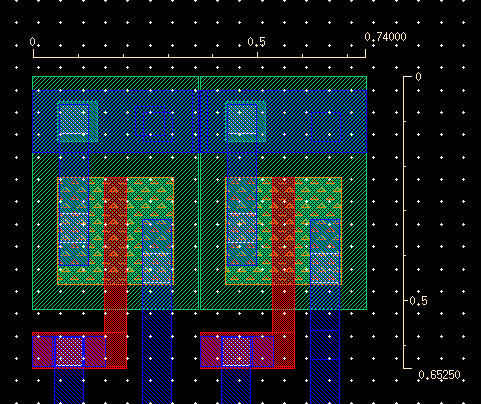
\includegraphics[width=7cm]{final_cells/BUF_PMOS}
  \caption{BUF Pull-up Network}
\label{fig:BUF_pmos}}
\qquad
\begin{minipage}{7cm}
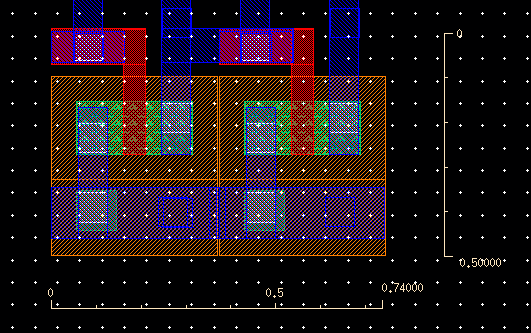
\includegraphics[width=7cm]{final_cells/BUF_NMOS}
  \caption{BUF Pull-down Network}
\label{fig:BUF_nmos}
\end{minipage}
\end{figure}

\begin{figure}[ht]
\centering
\parbox{8cm}{
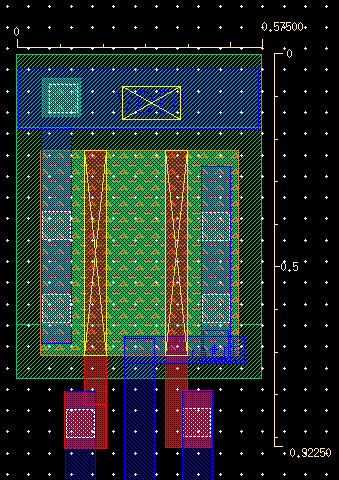
\includegraphics[width=7cm]{final_cells/NOR2_PMOS}
  \caption{NOR2 Pull-up Network}
\label{fig:NOR2_pmos}}
\qquad
\begin{minipage}{7cm}
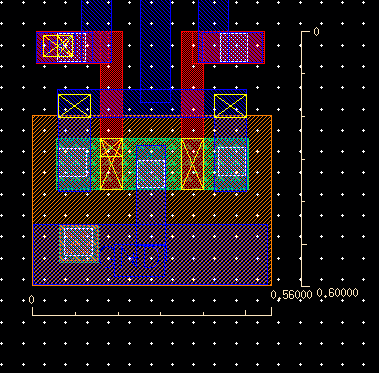
\includegraphics[width=7cm]{final_cells/NOR2_NMOS}
  \caption{NOR2 Pull-down Network}
\label{fig:NOR2_nmos}
\end{minipage}
\end{figure}

\begin{figure}[ht]
\centering
\parbox{8cm}{
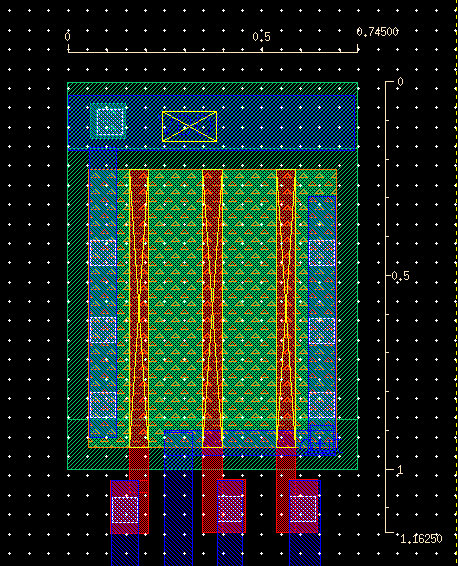
\includegraphics[width=7cm]{final_cells/NOR3_PMOS}
  \caption{NOR3 Pull-up Network}
\label{fig:NOR3_pmos}}
\qquad
\begin{minipage}{7cm}
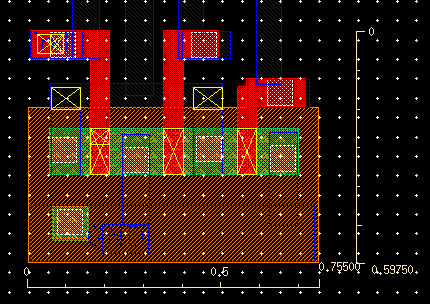
\includegraphics[width=7cm]{final_cells/NOR3_NMOS}
  \caption{NOR3 Pull-down Network}
\label{fig:NOR3_nmos}
\end{minipage}
\end{figure}

\begin{figure}[ht]
\centering
\parbox{8cm}{
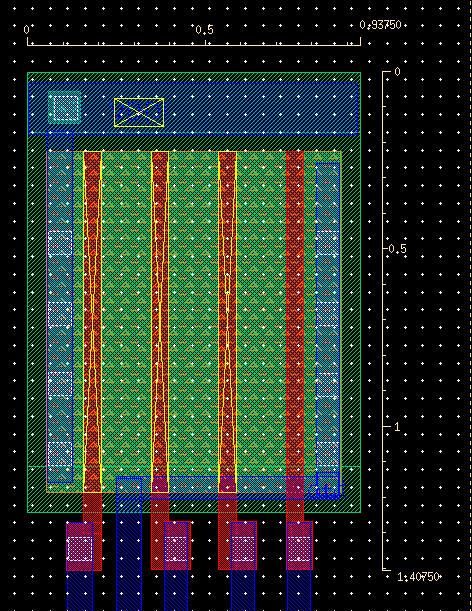
\includegraphics[width=7cm]{final_cells/NOR4_PMOS}
  \caption{NOR4 Pull-up Network}
\label{fig:NOR4_pmos}}
\qquad
\begin{minipage}{7cm}
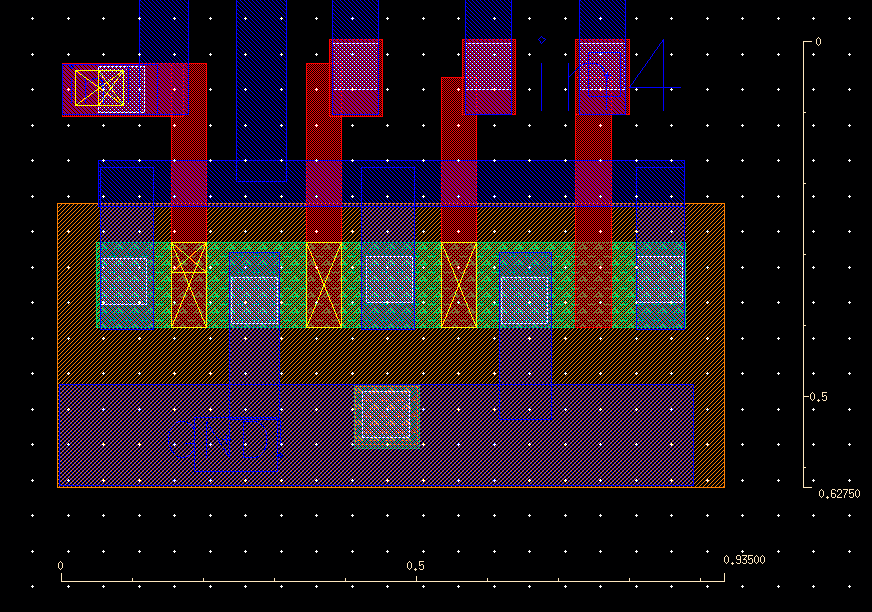
\includegraphics[width=7cm]{final_cells/NOR4_NMOS}
  \caption{NOR4 Pull-down Network}
\label{fig:NOR4_nmos}
\end{minipage}
\end{figure}

\begin{figure}[ht]
\centering
\parbox{8cm}{
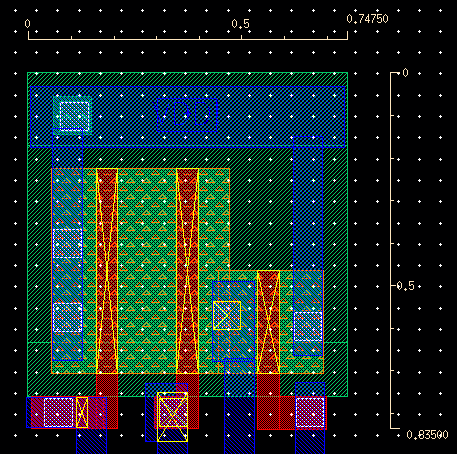
\includegraphics[width=7cm]{final_cells/OAI21_PMOS}
  \caption{OAI21 Pull-up Network}
\label{fig:OAI21_pmos}}
\qquad
\begin{minipage}{7cm}
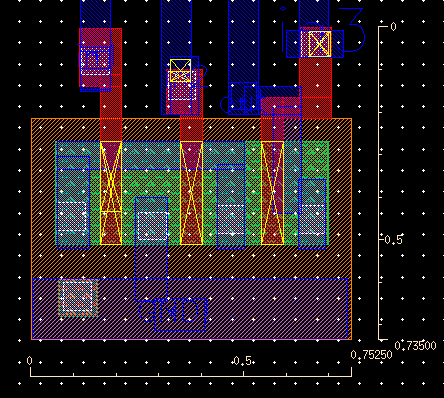
\includegraphics[width=7cm]{final_cells/OAI21_NMOS}
  \caption{OAI21 Pull-down Network}
\label{fig:OAI21_nmos}
\end{minipage}
\end{figure}

\begin{figure}[ht]
\centering
\parbox{8cm}{
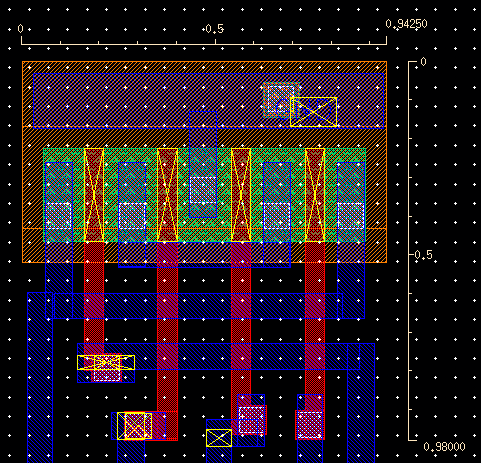
\includegraphics[width=7cm]{final_cells/OAI22_PMOS}
  \caption{OAI22 Pull-up Network}
\label{fig:OAI22_pmos}}
\qquad
\begin{minipage}{7cm}
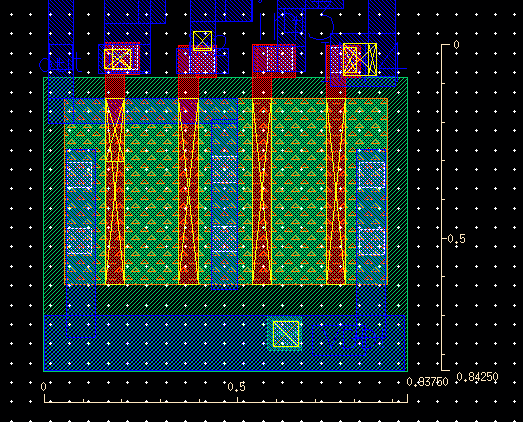
\includegraphics[width=7cm]{final_cells/OAI22_NMOS}
  \caption{OAI22 Pull-down Network}
\label{fig:OAI22_nmos}
\end{minipage}
\end{figure}

\begin{figure}[ht]
\centering
\parbox{8cm}{
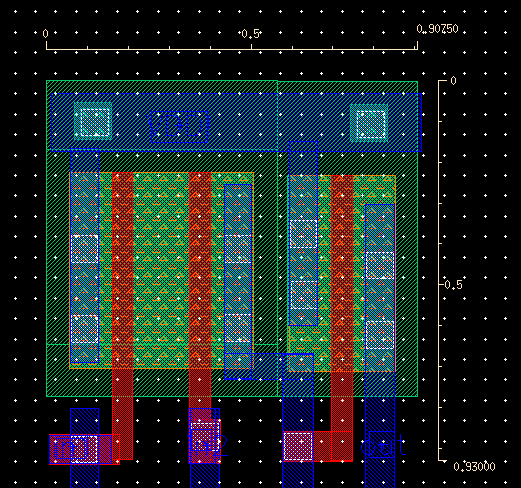
\includegraphics[width=7cm]{final_cells/OR2_PMOS}
  \caption{OR2 Pull-up Network}
\label{fig:OR2_pmos}}
\qquad
\begin{minipage}{7cm}
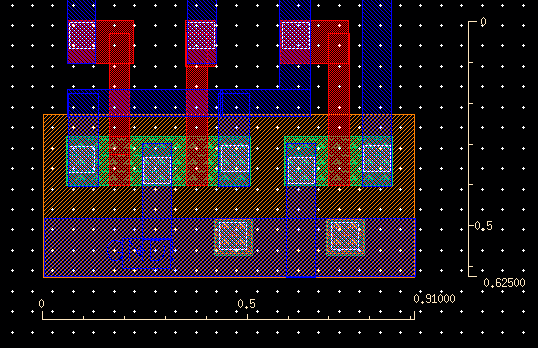
\includegraphics[width=7cm]{final_cells/OR2_NMOS}
  \caption{OR2 Pull-down Network}
\label{fig:OR2_nmos}
\end{minipage}
\end{figure}

\begin{figure}[ht]
\centering
\parbox{8cm}{
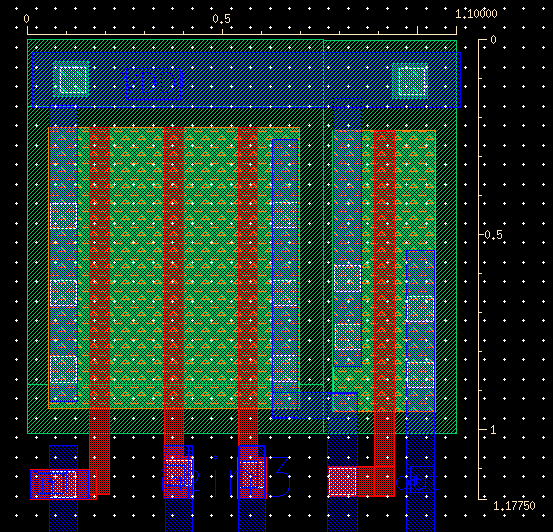
\includegraphics[width=7cm]{final_cells/OR3_PMOS}
  \caption{OR3 Pull-up Network}
\label{fig:OR3_pmos}}
\qquad
\begin{minipage}{7cm}
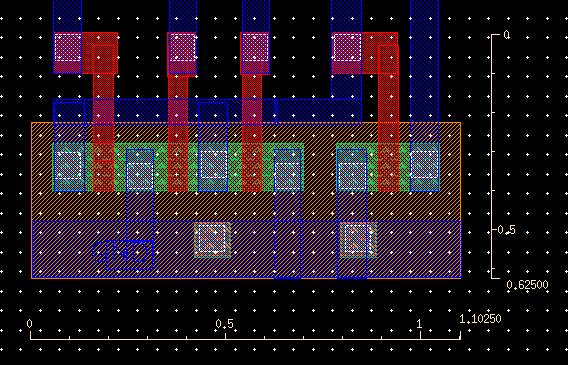
\includegraphics[width=7cm]{final_cells/OR3_NMOS}
  \caption{OR3 Pull-down Network}
\label{fig:OR3_nmos}
\end{minipage}
\end{figure}

\begin{figure}[ht]
\parbox{8cm}{
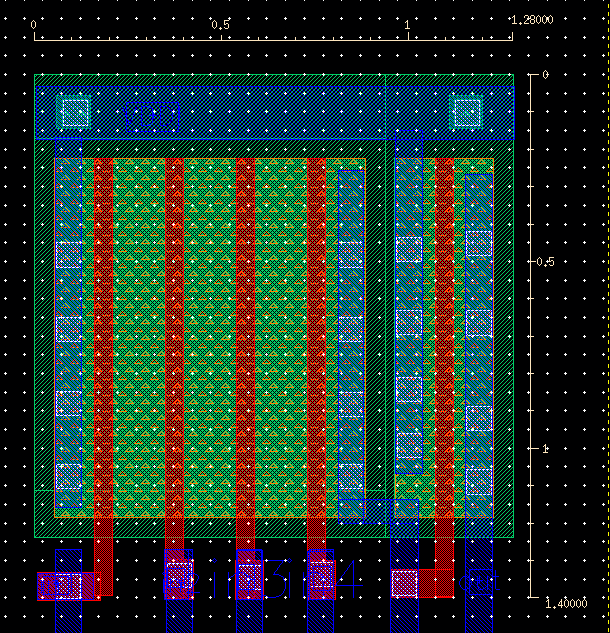
\includegraphics[width=7cm]{final_cells/OR4_PMOS}
  \caption{OR4 Pull-up Network}
\label{fig:OR4_pmos}}
\qquad
\begin{minipage}{7cm}
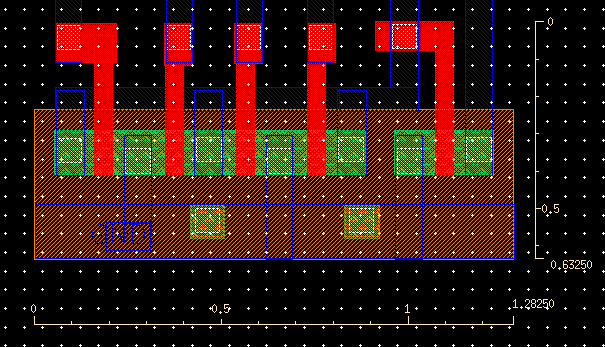
\includegraphics[width=7cm]{final_cells/OR4_NMOS}
  \caption{OR4 Pull-down Network}
\label{fig:OR4_nmos}
\end{minipage}
\end{figure}

\clearpage
\newpage
\bibliographystyle{plain}
\bibliography{vlsi}
\newpage
\end{document}
